\documentclass[12pt, letterpaper]{article}
\usepackage{makecell}
\usepackage{graphicx}
\usepackage{float}
\begin{document}

% Remove page numbers from title page and TOC
\pagestyle{empty}

\tableofcontents
\listoftables
\listoffigures
\newpage

% Begin page numbering here
\pagenumbering{arabic}
\pagestyle{plain}

\section*{The Requirement Specification}
\addcontentsline{toc}{section}{The Requirement Specification}
Our requirements, in order of priority, are: developing a fully functional web application, connecting a media platform to enable song manipulation, designing a BriForm-like page for music education, managing user login credentials, and grading music assignments. We decided on these requirements by listening to feedback from professors and music theory students on their experiences with BriForm.

\textbf{Application.} Having a working application, a way for users to interact with our product, is our number one priority. We plan to deliver a fully functional web application that users can access from anywhere. Our web app will host our BriForm-like tool, allowing teachers and students to complete assignments and study music.

\textbf{Media.} Our project is a music education tool. Thus, our users need a way to import songs so that they can study music and learn from it. We are choosing to use YouTube's API, which allows users to select a video on YouTube and then analyze it, dissect it, and overall hone their skills.

\textbf{Design.} The number one complaint that BriForm users possess is how clunky and unusable the design feels. We plan to keep the functionality of BriForm while updating the UI to be intuitive for users. We want people to enjoy using our tool, rather than it being a chore. Alongside a better UI, we plan to add some more functionality to our tool so that users can take their music education to the next level.

\textbf{Login.} Users will need a way to log in to our web application to save their projects and access them from any device. We are still figuring out the best way to store user credentials; however, we plan to create a login page so that users can securely store their projects.

\textbf{Grading.} Allowing teachers to set assignments and grade through our platform would make teachers' lives easier. It would provide a strong incentive to use our tool over an alternative such as BriForm. By allowing teachers to set up automatic grading for assignments it will give students faster feedback on their progress and take a load off teachers’ shoulders.

Overall, our requirements give us a clear focus when creating our music education tool. Our requirements are carefully chosen by feedback from teachers and students, and give us a path towards designing a music education tool that people will enjoy using.

\section*{Technical Approach}
\addcontentsline{toc}{section}{Technical Approach}
\subsection*{Project Space}
\addcontentsline{toc}{subsection}{Project Space}
Our project space consists of a frontend and backend space, as well as a synchronization method. The frontend space primarily consists of NextJS code. Each site component will have an individual file that defines it. Those components are then compiled into pages, with each page having its own folder and page.tsx file. The frontend space defines what the user is able to do on the site and how the user interface will facilitate it. 

The backend space will hold necessary user information, including login credentials, account type, classes enrolled/teaching, assignments or projects, etc. We need to have user accounts to fulfill our user requirements, so a strong backend is crucial. Whether we use a simpler approach with an external account system or a more customized approach with a backend provider, we will need to connect the back and front ends seamlessly with NextJS.

This project involves splitting of work among the group members. This necessitates a way to centralize and synchronize our work. We use GitHub to accomplish this. GitHub allows us to constantly have a “most recent” version of the site. It also ensures that any conflict caused by our separate work is quickly resolved and provides accountability for everyone committing their sections of the work themselves.

\subsection*{Functional Decomposition}
\addcontentsline{toc}{subsection}{Functional Decomposition}
\begin{figure}[H]
    \centering
    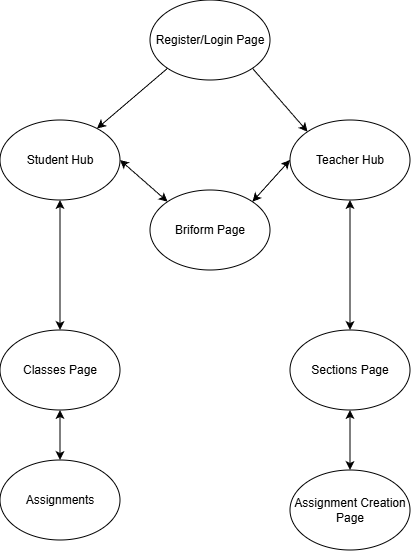
\includegraphics[width=0.5\linewidth]{images/401Technical.drawio.png}
    \caption{Technical Diagram}
    \label{fig:tech401}
\end{figure}
The first functional unit of the website is the register and login page. On this page, the user will be prompted to either log in to an existing account or to create a new account. If a user needs to create an account, they will be directed to do so while selecting whether they are a teacher or a student, and then will be redirected to the appropriate landing page. If a user already has an account and logs in, they will also be redirected to the appropriate landing page.

The student hub of our site is going to be where students end up after they log in. This will contain all of their classes as well as any assignments that are soon due. It will also have a redirect to the briform style page in case they want to make something independent from their classes. They will be able to view any saved projects they have completed, as well as be able to manage them.

From the student hub, students will be able to access their individual classes through the classes page. This will allow them to go into their classes and see anything that has been posted by the instructor, as well as any lessons they need to complete.

Via the classes page, students will be able to move to an assignment page in order to be able to see all assignments for that class, as well as their due dates and any grades if the assignments have been graded.

When it comes to teachers, after logging in, they will be sent to the teacher hub. In this hub, they will be able to view all classes they are currently running, as well as being able to make new classes. They can also directly access the briform style page from here as well if they want to use the tool and create new projects, as well as save them. Teachers will also be able to access the sections page from the teacher hub.

The sections page is a per-class page that lets the teacher manage that class. From here, they can post announcements or other class-related posts. They will also be able to create sections that, when the students are on the classes page, they will be able to view the sections the teachers create. In these sections teacher can post material for students to learn from. The last thing the teacher can do on the sections page is to post and grade assignments for the students.

In the assignment creation page, the teacher will be able to make new assignments for their students to work on. These can be simple assignments, such as record and submit something, or more involved assignments where they have to use the Briform style tool to make and submit a project. When using the assignment creation page, the teacher can also set up how the assignment is going to be graded. They can decide whether the assignment will be graded automatically or if it will be manually graded by them after the students submit.

Finally, we have a Briform-style page that takes inspiration from the site Briformer. In this page, students and teachers will be able to make new projects in which they use a music audio file or a video to score the music and practice things like ear theory. They will also have the choice to save the project they finished, and if they want to continue a project, they can upload an existing saved project to resume where they left off.

\subsection*{Key Design Decisions}
\addcontentsline{toc}{subsection}{Key Design Decisions}
There are several key design decisions we need to make throughout the process of this project. There are two major decisions surrounding the project space. The first is whether to use a web-based approach with NextJS (or similar language) or an application-based approach with a language like Python. Another decision is whether to use an external account system (such as using exclusively a YouTube/Google account) or a back-end like Supabase.

The rest of the major decisions deal with the design and structure of the program. The first is deciding whether we want to use a design inspired by Briform or make our own design that accomplishes similar functionality. We must also consider if and how we want to integrate Spotify and/or YouTube, as well as how both can be used. The last major decision is whether to support some form of auto-grading of assignments or if grading must be strictly manual from instructors.

\section*{Design Concepts, Evaluation, and Selection}
\addcontentsline{toc}{section}{Design Concepts, Evaluation, and Selection}
\subsection*{Web Application vs. Downloadable Application - Davis Akard}
\addcontentsline{toc}{subsection}{Web Application vs. Downloadable Application - Davis Akard}
When we first began crafting our design for a music education tool, we deliberated between two ways to bring it to users. We could either design a web application that users could connect to through a browser or make an executable that users would download and launch. Both ideas had their pros and cons; however, we ultimately decided on designing a web application. We went this route for multiple reasons, but the biggest reason was usability. One of our main focuses is usability, and a web application is much more usable than a downloaded application. Web browsers give users access to our tool by simply clicking on a link, whereas a downloaded application is harder to distribute, requires downloading, and is overall clunkier to use. We also decided on a web browser because it was a format that we were more comfortable with designing, implementing, and coding. HTML, CSS, and JavaScript are all relatively basic programming languages and something that we are either comfortable with or will become comfortable with quickly. Designing a downloadable application is something we are unfamiliar with, and designing one would take a lot more effort than a web application.

\subsection*{Offsite Login vs. Backend Provider - Ryan Thweatt}
\addcontentsline{toc}{subsection}{Offsite Login vs. Backend Provider - Ryan Thweatt}
Another important decision to make is how we want to handle the account system. We could use an exclusively external account system. This would involve taking advantage of existing accounts with the platform(s) we integrate into the app (eg., YouTube/Google or Spotify accounts). This would be very simple for users, as it is a common method of account creation. However, it does not allow for the same level of customization that using a backend provider like Supabase would. Using a backend provider would likely make it simpler to differentiate between student and instructor accounts and give us more flexibility in how we design the front end. In addition, we could link multiple offsite accounts (i.e., link both YouTube and Spotify accounts) to a user’s profile instead of being locked into one.

\subsection*{Auto-Grading \& Manual Grading vs. Strictly Manual Grading - Viktor Potter}
\addcontentsline{toc}{subsection}{Auto-Grading \& Manual Grading vs. Strictly Manual Grading - Viktor Potter}
One of the major design decisions for our product was whether assignments could be marked as autograded or manually graded by teachers, or if we would require teachers to grade their assignments with no option for autograding. For the choice of making teachers grade themselves with no option for autograding, it will be as simple as providing the teacher a box where they put the total possible score when creating an assignment, and then having them go back once a student submits an assignment to put in a grade themselves. When it comes to having an autograde system, we would have to make our own model for how assignments should be graded, as well as implement a way for teachers to adjust the autograding system. When it comes to these two alternatives for grading, the best decision for what we are making would be to only have manual grading enabled. As the time for our project is limited and along with all of the other functions that need to be built for the website, the time it would take to set up a proper autograding system would be too high compared to its overall importance to the project. The autograding feature may also be something that could cause teachers' headaches if we do not implement it properly, or if there are bugs within the autograding system that we fail to find. The time that would be spent making this feature would be utilized much better for optimizing the main components of the site and enhancing the user experience through a well-polished site instead of an autograding system.

\subsection*{Spotify Integration vs. YouTube Integration - Connor Finley}
\addcontentsline{toc}{subsection}{Spotify Integration vs. YouTube Integration - Connor Finley}
When considering how to allow users to import music into our application, we debated between integrating Spotify or YouTube.  With what work we have done thus far, we have discovered some pros and cons about Spotify in particular.  Spotify's API is extremely intuitive, and account login is simple through OAuth.  However, Spotify's API does not allow for streaming full songs, which is a major drawback for our application.  On the other hand, YouTube's API allows for full video streaming, which is perfect for our use case.  Though we have not experimented with YouTube's API yet, we believe that the benefits of full video streaming outweigh the drawbacks of learning a new API.  Therefore, we have decided to integrate YouTube into our application for use with Briform.  While it may seem like the time investment to integrate Spotify's API went to waste, we still plan to use it in combination with a Spotify preview finder API to pull 30-second preview clips that can we used for the song-to-score functionality of our application.  By using these two APIs in tandem, we believe that we can provide a seamless experience for users to import music into our application.

\section*{Deliverables}
\addcontentsline{toc}{section}{Deliverables}
Our project deliverables can be divided into three main phases: Development, Testing/Feedback, and Deployment.  The specific deliverables for each category are outlined below:

\subsection*{Development}
\addcontentsline{toc}{subsection}{Development}
\begin{itemize}
    \item[--] Implement account structure using Supabase and integrate these accounts with YouTube/Spotify accounts
    \item[--] Complete "Neo-Briform" tool that allows students to diagram form and phrase structure in a more intuitive and user-friendly way than Briform
    \item[--] Complete song-to-score functionality that allows students to test their ear training skills against music that they are familiar with
\end{itemize}

\subsection*{Testing/Feedback}
\addcontentsline{toc}{subsection}{Testing/Feedback}
\begin{itemize}
    \item[--] Select a preliminary test group of students to use the tool and provide feedback
    \item[--] Create a Google Form that test users can fill out to provide feedback on the tool
    \item[--] Conduct at least one round of testing and feedback collection from the preliminary test group
    \item[--] Use given feedback to improve the tool and fix any bugs or issues that arise
\end{itemize}

\subsection*{Deployment}
\addcontentsline{toc}{subsection}{Deployment}
\textit{Note: These tasks will mostly fall on Connor as he has important connections in the College of Music}
\begin{itemize}
    \item[--] Coordinate meetings with Theory Department head and other relevant faculty to present the tool and discuss its use cases in our curriculum
    \item[--] If necessary, make any final adjustments to the tool based on faculty feedback
    \item[--] Potentially coordinate meeting with Dean of the College of Music to discuss launching the tool
\end{itemize}

\section*{Project Management}
\addcontentsline{toc}{section}{Project Management}
The timeline below includes major milestones and expected completion time frames.  It is important to note that this timeline does not give specific expectations but simply serves as a baseline expectation for how we will progress.

\subsection*{Proposed Project Timeline}
\addcontentsline{toc}{subsection}{Proposed Project Timeline}
\textit{Note: The bold lines in the table serve to separate our milestones into three main phases: Development, Testing/Feedback, and Deployment}
\begin{table}[h!]
\caption{Proposed Project Timeline}
\centering
\begin{tabular}{|p{8cm}|p{4cm}|}
\hline
\textbf{Milestone} & \textbf{Target Date} \\
\Xhline{4\arrayrulewidth}
Basic implementation of Briform clone and score reduction functionality & End of January \\
\hline
Continued work on refining tool and preparing for testing & Early/Mid February \\
\Xhline{4\arrayrulewidth}
Preliminary test group is selected and asked to complete an assignment that utilizes the tool & End of February \\
\hline
Begin improving tool based on feedback received from test group & Spring Break \\
\Xhline{4\arrayrulewidth}
Continue improving based on feedback and desired features and begin communicating with College of Music faculty & Early April \\
\hline
Fix remaining bugs, polish features, and continue communications with College of Music faculty & Mid/Late April \\
\hline
Production Ready & Early May \\
\hline
\end{tabular}
\end{table}

\section*{Budget}
\addcontentsline{toc}{section}{Budget}
Because we have no financial costs associated with our project, our budget will outline how much time we expect to allocate towards specific tasks.  Our goal is to work 30-40 hours per week until completion.  In the table below, our estimated workload is shown as a percentage of our weekly expectation, and three perecentages are listed for each of the three phases of our project.  

\subsection*{Estimated Budget}
\addcontentsline{toc}{subsection}{Estimated Budget}
\begin{table}[h!]
\caption{Estimated Budget}
\centering
\begin{tabular}{|p{6cm}|p{6cm}|}
\hline
\textbf{Tasks} & \textbf{Expected Workload (\%)} \\
\hline
Development Deliverables & 1: 90\%, 2: 40\%, 3: 10\% \\
\hline
Feedback Deliverables & 1: 10\%, 2: 60\%, 3: 10\% \\
\hline
Deployment Deliverables & 1: 00\%, 2: 00\%, 3: 80\%\\
\hline
\end{tabular}
\end{table}

\end{document}